\section{Binary Search Trees}

\subsection{Definition, Chapter 12}

\index{Binary Search Tree!Definition \S 12}

The linked data structure in which every node is an object has a $key$ and attributes $left$, $right$, and $p$ that point to the nodes of the left child, right child, and parent.  If the node does not have such an attribute, its value is \verb|NIL|.  The root node is the only node whose parent is \verb|NIL|.

\

Binary Search Tree Property.  Let $x$ be a node in a binary search tree.  If $y$ is a node in the left subtree of $x$, then $y.key \le x.key$.  If $y$ is a node in the right subtree of $x$, then $x.key \le y.key$.  

Note that it doesn't just apply to the children of $x$, but any nodes in the subtree rooted at $x$.  

\

Operations, with $n$ being the number of nodes and $h$ being the height of the tree, $\log_2 n \le h \le n$.  The best case for $h$ is that the tree is balanced, with $h = \log_2 n$, and the worst case is that the tree is a linear chain of $n$ nodes, $h = n$.  

\

\begin{tabular}{>{\sc }l >{$}c<{$}}
	Inorder-Tree-Walk & \Theta(n) \cr
	Tree-Search & O(n) \cr
	Tree-Minimum & O(h) \cr
	Tree-Maximum & O(h) \cr
	Tree-Successor & O(h) \cr
	Tree-Predecessor &O(h) \cr
	Tree-Insert & O(h) \cr
	Tree-Delete & O(h) \cr
\end{tabular}

%%%%%%%
\subsection{Old Exam Questions}
%%%%%
\subsubsection{S15 \#S9}

	% S15 \#S9
	Mark true/false against the following statements. 
	\begin{enumerate}[label=\alph*.]
		\item (Same as F15 \#S7a) A binary search tree of size $N$ will always find a key in at most $O(\log N)$ time.
		\item (Same as F15 \#S5c) A breadth first search algorithm can be considered as a special case of heuristic search algorithm.
		\item (Same as F15 \#Sb)  An optimal binary search tree is not necessarily a balanced tree.
		\item A dynamic programming approach uses top-down problem solving strategy to solve optimization problem.
	\end{enumerate}

\subsubsection{Solutions}

\begin{enumerate}[label=\alph*.]
	\item False.  A binary search tree of height $h$ will always find a key in at most $O(h)$ time.  In a {\it balanced} binary search tree, the height is about $\log N$, so the statement is true for balanced trees, but a binary search tree can also be a linear chain with height $N$, so the search could take up to $O(N)$ time.  
	\item No idea.  We didn't cover heuristics, and it's not in the textbook.
	\item True.  
	\item True.  One dynamic programming approach uses a top-down problem solving with memoization strategy, and another uses bottom-up problem solving.  
\end{enumerate}

\subsubsection{F15 \#S7}

Parts (a) and (b) the same as (a) and (c) above.  

	% F15 #S7
	Mark True or False against the following statements.
	\begin{enumerate}[label=\alph*.]
		\item  (Same as S15 \#9a) A binary search tree of size $N$ will always find a key in at most $O(\log N)$ time.
		\item An optimal binary search is not necessary a balanced tree.
		\item A binary heap always maintains a balanced tree as practical as it can be.
		\item To implement a priority queue binomial heap is preferred over binary heap.
		\item A graph formed by strongly connected components, a strongly connected components graph (SCC) is always a minimum spanning tree.  
	\end{enumerate}
	
\subsubsection{Solutions}

\begin{enumerate}[label=\alph*.]
	\item False.  If the tree is balanced, yes.  If not, it could be up to $O(n)$ time.  
	\item True.  
	\item True-ish.  A binary heap is a balanced tree.  Not ``as practical as it can be.''  Just is.  
	\item No idea.  Not in our textbook.  ``Binomial heap'' is in an exercise, but no priority queue binomial heap.
	\item False.  A strongly connected graph is a spanning tree, but not necessarily a minimal spanning tree.  
\end{enumerate}
	

\subsubsection{F16 \#S8, First part, Same as above}
	% F16 #S8
	Mark true/false (T/F) against the following statements.  
	
	[Note that the subquestions were not enumerated in the original.  I enumerated them so I could write the solutions and justifications separately.  ]
	
	\begin{enumerate}
		\item A binary search tree of size $N$ will always find a key at most $O(\lg N)$ time
		\item A breadth first search can be considered as a special case of heuristic search algorithm.
		\item An optimal binary search tree is not necessarily being a balanced tree.
		\item A dynamic programming approach uses top-down problem solving strategy to solve optimization problem.
	\end{enumerate}
	
\subsubsection{Solutions}

\begin{enumerate}
	\item False.  A balanced binary search tree will always find a tree in at most $O(\lg N)$ time, but a binary search tree does not have to be balanced.  In the worst case, if the tree is just one branch, it would require $O(N)$ time.  
	\item No idea.  This book doesn't cover heuristics, and we didn't talk about it in class.  
	\item True.  
	\item True, if the question means, ``There is a dynamic programming approach that uses a top-down decision strategy...''  
	
	False if the question means, ``A dynamic programming approach must use a top-down problem solving stragegy...''  or ``The dynamic programming approach uses the top-down problem solving strategy...''
	
	The question statement is missing an article preceding ``top-down programming approach,'' so I will not trust my grade to interpretations of the subtleties of the use of another article in the sentence.
	
	Dynamic programming can use either top-down with memoization or bottom-up.  
\end{enumerate}



%%%%%%%%%%%%%%%%%%%%%%%
\section{Optimal Binary Search Tree}

\index{Binary Search Tree!Optimal!Definition, \S 15.5}
\index{Dynamic Programming!Chain Matrix Multiplication!see {Binary Search Tree, Optimal}}
\index{Binary Search Tree!Optimal!see {Dynamic Programming, Chain Matrix Multiplication}}

\subsection{Definition, \S 15.5}

A tree whose expected search cost is smallest.  

\

\begin{itemize}
	\item A set of $n$ {\it distinct} keys in sorted order, $K = (k_1, k_2, \dots, k_n)$ with $k_1 < k_2 < \cdots < k_n$
	\item For each key $k_i$, a probability $p_i$ that a search will be for $k_i$.  
	\item A set of $n+1$ dummy keys $d_0, d_1, \dots d_n$ representing values not in $K$, such that $d_0$ represents anything less than $k_1$, $d_1$ represents anything between $k_1$ and $k_2$, $\dots$, and $d_n$ represents anything greater than $k_n$.  
	\item For each key $d_i$, a probability $q_i$ that the search will correspond to $d_i$.  
	\item Each $d$ node is a leaf; each $k$ node is internal.  

$$\sum_{i=1}^n p_i + \sum_{i=0}^n q_i = 1$$

	\item Given a binary search tree $T$, the cost of a search is the number of nodes examined, which is one more than the depth of the node found by the search.
	
\begin{align*}
	E[\text{Search cost in $T$}] &= \sum_{i=1}^n (\text{depth}_T(k_i) + 1) \cdot p_i + \sum_{i=0}^n (\text{depth}_T(d_i) + 1) \cdot q_i \cr
	&= \sum_{i=1}^n \text{depth}_T(k_i) \cdot p_i + \sum_{i=1}^n p_i + \sum_{i=0}^n \text{depth}_T (d_i) \cdot q_i + \sum_{i=0}^n q_i \cr
	&= 1 + \sum_{i=1}^n \text{depth}_T(k_i) \cdot p_i + \sum_{i=0}^n \text{depth}_T (d_i) \cdot q_i\cr
	\cr
\end{align*}

\end{itemize}

\subsection{Brad's Example}

Unlike the examples in the text, I made all of the probabilities different, making sure their sum is 1.00.

\

\begin{tabular}{ >{$}c<{$} | *7{c} }
	i & 0 & 1 & 2 & 3 & 4 & 5 \cr\hline
	p_i & & 0.10 & 0.11 & 0.12 & 0.13 & 0.15 \cr
	q_i & 0.04 & 0.05 & 0.06 & 0.07 & 0.08 & 0.09 \cr
\end{tabular}

\


\begin{tabular}{ >{$}c<{$} | *7{c} }
w & 0 & 1 & 2 & 3 & 4 & 5 \cr\hline
1 & 0.04  & 0.19  & 0.36  & 0.55  & 0.76  & 1.00  \cr
2 &  & 0.05  & 0.22  & 0.41  & 0.62  & 0.86  \cr
3 &  &  & 0.06  & 0.25  & 0.46  & 0.70  \cr
4 &  &  &  & 0.07  & 0.28  & 0.52  \cr
5 &  &  &  &  & 0.08  & 0.32  \cr
6 &  &  &  &  &  & 0.09  \cr
\end{tabular}

\

There is only one way to construct the subtree containing only one of the $k$ nodes.  

\

%%%
\begin{tabular}{p{3in}p{3in}}

\

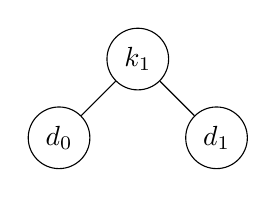
\begin{tikzpicture}[x=10mm, y=10mm]
	\node [circle, draw] (k1) at (0,0) {$k_1$};
	\node [circle, draw] (d0) at (-1,-1) {$d_0$};
	\node [circle, draw] (d1) at (1,-1) {$d_1$};
	\foreach \from/\to in {k1/d0, k1/d1}
		\draw (\from) -- (\to);
\end{tikzpicture}

$1\times (p_1) + 2\times (q_0 + q_1)$

$= (q_0) + (q_1) + (p_1 + q_0 + q_1)$

${\color{red}= e[1,0] + e[2,1] + w[1,1]}$

${\color{blue}= 0.28 \to e[1,1]}$

$1 \to root[1,1]$


&

\

${\color{red}w[1,1] =  0.19}$

\

\begin{tabular}{ >{$}c<{$} | *7{c} }
e & 0 & 1 & 2 & 3 & 4 & 5 \cr\hline
1 & \color{red} 0.04  & \color{blue} 0.28  \cr %& 0.70  & 1.21  & 1.89  & 2.70  \cr
2 &  & \color{red} 0.05  \cr % & 0.33  & 0.81  & 1.38  & 2.16  \cr
3 &  &  & 0.06 \cr %  & 0.38  & 0.92  & 1.57  \cr
4 &  &  &  & 0.07 \cr %  & 0.43  & 1.04  \cr
5 &  &  &  &  & 0.08 \cr %  & 0.49  \cr
6 &  &  &  &  &  & 0.09  \cr
\end{tabular}

\begin{tabular}{ >{$}c<{$} | *7{c} }
root & 1 & 2 & 3 & 4 & 5 \cr\hline
1 & 1  \cr % & 2  & 2  & 3  & 4  \cr
%2 &  & 2  & 3  & 3  & 4  \cr
%3 &  &  & 3  & 4  & 4  \cr
%4 &  &  &  & 4  & 5  \cr
%5 &  &  &  &  & 5  \cr
\end{tabular}

\cr
\end{tabular}

\

%%%
\begin{tabular}{p{3in}p{3in}}

\

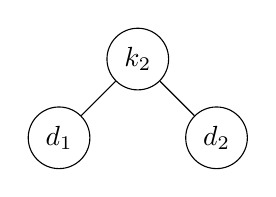
\begin{tikzpicture}[x=10mm, y=10mm]
	\node [circle, draw] (k2) at (0,0) {$k_2$};
	\node [circle, draw] (d1) at (-1,-1) {$d_1$};
	\node [circle, draw] (d2) at (1,-1) {$d_2$};
	\foreach \from/\to in {k2/d1, k2/d2}
		\draw (\from) -- (\to);
\end{tikzpicture}

$1\times (p_2) + 2\times (q_1 + q_2)$

$= (q_1) + (q_2) + (p_2 + q_1 + q_2)$

${\color{red}= e[2,1] + e[3,2] + w[2,2]}$

${\color{blue}= 0.33 \to e[2,2]}$

$2 \to root[2,2]$


&

\

${\color{red}w[2,2] =  0.19}$

\

\begin{tabular}{ >{$}c<{$} | *7{c} }
e & 0 & 1 & 2 & 3 & 4 & 5 \cr\hline
1 & 0.04  & 0.28  \cr %& 0.70  & 1.21  & 1.89  & 2.70  \cr
2 &  & \color{red} 0.05   &  \color{blue} 0.33 \cr % & 0.81  & 1.38  & 2.16  \cr
3 &  &  & \color{red} 0.06 \cr %  & 0.38  & 0.92  & 1.57  \cr
4 &  &  &  & 0.07 \cr %  & 0.43  & 1.04  \cr
5 &  &  &  &  & 0.08 \cr %  & 0.49  \cr
6 &  &  &  &  &  & 0.09  \cr
\end{tabular}

\begin{tabular}{ >{$}c<{$} | *7{c} }
root & 1 & 2 & 3 & 4 & 5 \cr\hline
1 & 1  \cr % & 2  & 2  & 3  & 4  \cr
2 &  & 2 \cr %  & 3  & 3  & 4  \cr
%3 &  &  & 3  & 4  & 4  \cr
%4 &  &  &  & 4  & 5  \cr
%5 &  &  &  &  & 5  \cr
\end{tabular}

\cr
\end{tabular}

\

...and so forth.  

\

%%%
\begin{tabular}{p{3in}p{3in}}

\

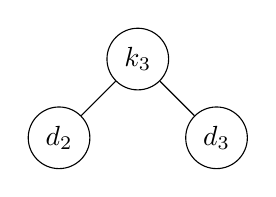
\begin{tikzpicture}[x=10mm, y=10mm]
	\node [circle, draw] (k2) at (0,0) {$k_3$};
	\node [circle, draw] (d1) at (-1,-1) {$d_2$};
	\node [circle, draw] (d2) at (1,-1) {$d_3$};
	\foreach \from/\to in {k2/d1, k2/d2}
		\draw (\from) -- (\to);
\end{tikzpicture}


\

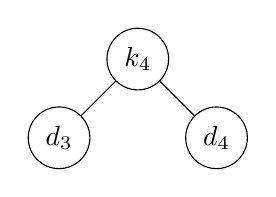
\begin{tikzpicture}[x=10mm, y=10mm]
	\node [circle, draw] (k2) at (0,0) {$k_4$};
	\node [circle, draw] (d1) at (-1,-1) {$d_3$};
	\node [circle, draw] (d2) at (1,-1) {$d_4$};
	\foreach \from/\to in {k2/d1, k2/d2}
		\draw (\from) -- (\to);
\end{tikzpicture}


\

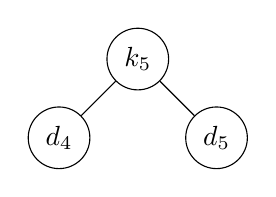
\begin{tikzpicture}[x=10mm, y=10mm]
	\node [circle, draw] (k2) at (0,0) {$k_5$};
	\node [circle, draw] (d1) at (-1,-1) {$d_4$};
	\node [circle, draw] (d2) at (1,-1) {$d_5$};
	\foreach \from/\to in {k2/d1, k2/d2}
		\draw (\from) -- (\to);
\end{tikzpicture}


&

\

\begin{tabular}{ >{$}c<{$} | *7{c} }
e & 0 & 1 & 2 & 3 & 4 & 5 \cr\hline
1 & 0.04  & 0.28  \cr %& 0.70  & 1.21  & 1.89  & 2.70  \cr
2 &  & 0.05   &   0.33 \cr % & 0.81  & 1.38  & 2.16  \cr
3 &  &  & 0.06  & 0.38  \cr % & 0.92  & 1.57  \cr
4 &  &  &  & 0.07  & 0.43 \cr %  & 1.04  \cr
5 &  &  &  &  & 0.08 & 0.49  \cr
6 &  &  &  &  &  & 0.09  \cr
\end{tabular}

\begin{tabular}{ >{$}c<{$} | *7{c} }
root & 1 & 2 & 3 & 4 & 5 \cr\hline
1 & 1  \cr % & 2  & 2  & 3  & 4  \cr
2 &  & 2 \cr %  & 3  & 3  & 4  \cr
3 &  &  & 3 \cr %  & 4  & 4  \cr
4 &  &  &  & 4 \cr %  & 5  \cr
5 &  &  &  &  & 5  \cr
\end{tabular}

\cr
\end{tabular}

\qquad

\



\

There are two ways to construct each of the subtrees containing two $k$ nodes.  Note how each of these subtrees contains one of the above subtrees.  Choose the option that gives the optimal subtree, {\it i.e} with the lowest expected cost.  

\

\hskip -.5in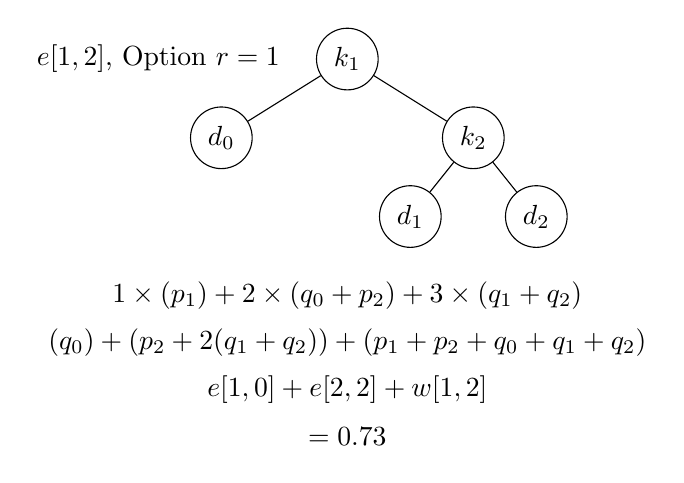
\begin{tikzpicture}[x=8mm, y=10mm]
	\node () at (-3,0) {$e[1,2]$, Option $r=1$};
	\node [circle, draw] (k1) at (0,0) {$k_1$};
	\node [circle, draw] (k2) at (2,-1) {$k_2$};
	\node [circle, draw] (d0) at (-2,-1) {$d_0$};
	\node [circle, draw] (d1) at (1,-2) {$d_1$};
	\node [circle, draw] (d2) at (3,-2) {$d_2$};
	\foreach \from/\to in {k1/d0, k1/k2, k2/d1, k2/d2}
		\draw (\from) -- (\to);
	\node () at (0,-3) {$1\times (p_1) + 2\times (q_0 + p_2) + 3 \times (q_1 + q_2) $};
	\node () at (0,-3.6) {$ (q_0) + (p_2 + 2(q_1 + q_2)) + (p_1 + p_2 + q_0 + q_1 + q_2)$};
	\node () at (0,-4.2) {$e[1,0] + e[2,2] + w[1,2] $};
	\node () at (0, -4.8) {$= 0.73$};
\end{tikzpicture}
\qquad
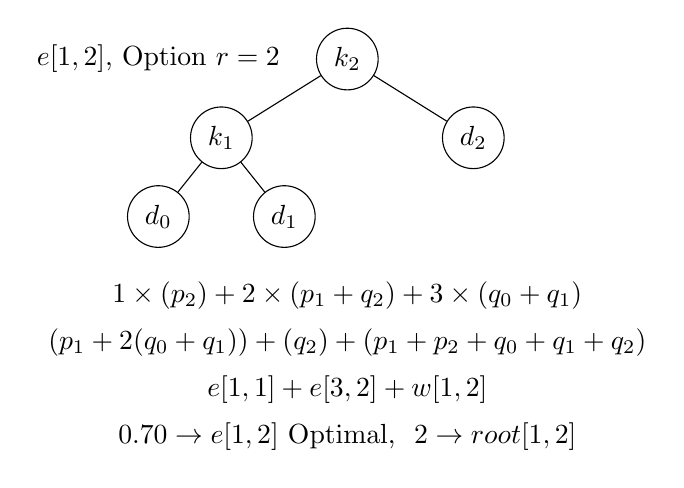
\begin{tikzpicture}[x=8mm, y=10mm]
	\node () at (-3,0) {$e[1,2]$, Option $r=2$};
	\node [circle, draw] (k1) at (-2,-1) {$k_1$};
	\node [circle, draw] (k2) at (0,0) {$k_2$};
	\node [circle, draw] (d0) at (-3,-2) {$d_0$};
	\node [circle, draw] (d1) at (-1,-2) {$d_1$};
	\node [circle, draw] (d2) at (2,-1) {$d_2$};
	\foreach \from/\to in {k2/k1, k2/d2, k1/d0, k1/d1}
		\draw (\from) -- (\to);
	\node () at (0,-3) {$1\times (p_2) + 2\times (p_1 + q_2) + 3 \times (q_0 + q_1) $};
	\node () at (0,-3.6) {$(p_1 + 2(q_0+q_1)) + (q_2) + (p_1 + p_2 + q_0 + q_1 + q_2)$};
	\node () at (0,-4.2) {$e[1,1] + e[3,2] + w[1,2]$};
	\node () at (0, -4.8) {$0.70 \to e[1,2]$ Optimal, \ $2 \to root[1,2]$};
\end{tikzpicture}

\

\hskip -.5in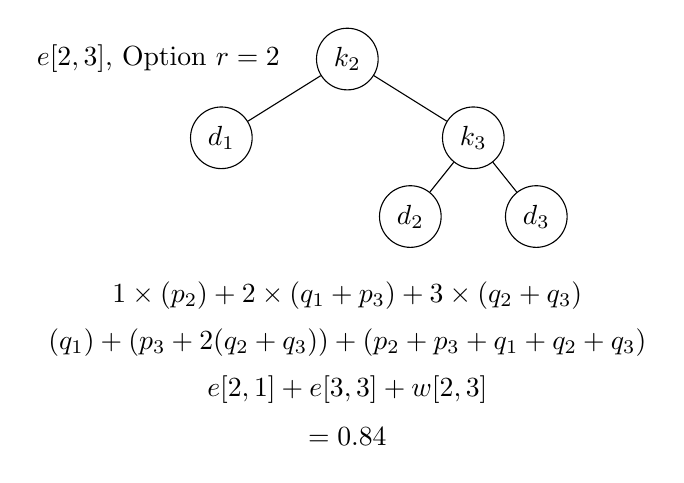
\begin{tikzpicture}[x=8mm, y=10mm]
	\node () at (-3,0) {$e[2,3]$, Option $r=2$};
	\node [circle, draw] (k2) at (0,0) {$k_2$};
	\node [circle, draw] (k3) at (2,-1) {$k_3$};
	\node [circle, draw] (d1) at (-2,-1) {$d_1$};
	\node [circle, draw] (d2) at (1,-2) {$d_2$};
	\node [circle, draw] (d3) at (3,-2) {$d_3$};
	\foreach \from/\to in {k2/d1, k2/k3, k3/d2, k3/d3}
		\draw (\from) -- (\to);
	\node () at (0,-3) {$1\times (p_2) + 2\times (q_1 + p_3) + 3 \times (q_2 + q_3)  $};
	\node () at (0,-3.6) {$ (q_1) + (p_3 + 2(q_2 + q_3)) + (p_2 + p_3 + q_1 + q_2 + q_3)$};
	\node () at (0,-4.2) {$e[2,1] + e[3,3] + w[2,3] $};
	\node () at (0, -4.8) {$= 0.84$};
\end{tikzpicture}
\qquad
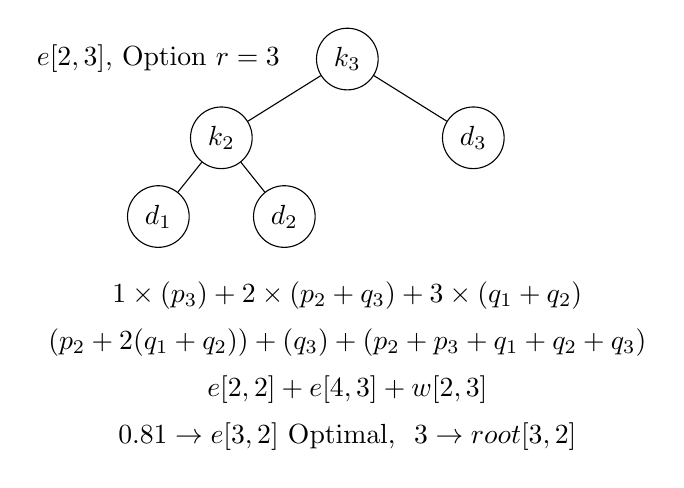
\begin{tikzpicture}[x=8mm, y=10mm]
	\node () at (-3,0) {$e[2,3]$, Option $r=3$};
	\node [circle, draw] (k2) at (-2,-1) {$k_2$};
	\node [circle, draw] (k3) at (0,0) {$k_3$};
	\node [circle, draw] (d1) at (-3,-2) {$d_1$};
	\node [circle, draw] (d2) at (-1,-2) {$d_2$};
	\node [circle, draw] (d3) at (2,-1) {$d_3$};
	\foreach \from/\to in {k3/k2, k3/d3, k2/d1, k2/d2}
		\draw (\from) -- (\to);
	\node () at (0,-3) {$1\times (p_3) + 2\times (p_2 + q_3) + 3 \times (q_1 + q_2)$};
	\node () at (0,-3.6) {$(p_2 + 2(q_1+q_2)) + (q_3) + (p_2 + p_3 + q_1 + q_2 + q_3)$};
	\node () at (0,-4.2) {$e[2,2] + e[4,3] + w[2,3]$};
	\node () at (0, -4.8) {$0.81 \to e[3,2]$ Optimal, \ $3 \to root[3,2]$};
\end{tikzpicture}

\

\begin{tabular}{ >{$}c<{$} | *7{c} }
e & 0 & 1 & 2 & 3 & 4 & 5 \cr\hline
1 & 0.04  & 0.28 & 0.70  \cr % & 1.21  & 1.89  & 2.70  \cr
2 &  & 0.05   &   0.33 & 0.81  \cr % & 1.38  & 2.16  \cr
3 &  &  & 0.06  & 0.38  & 0.92  \cr % & 1.57  \cr
4 &  &  &  & 0.07  & 0.43 & 1.04  \cr
5 &  &  &  &  & 0.08 & 0.49  \cr
6 &  &  &  &  &  & 0.09  \cr
\end{tabular}

\begin{tabular}{ >{$}c<{$} | *7{c} }
root & 1 & 2 & 3 & 4 & 5 \cr\hline
1 & 1  & 2  \cr % & 2  & 3  & 4  \cr
2 &  & 2  & 3  \cr % & 3  & 4  \cr
3 &  &  & 3 & 4   \cr %& 4  \cr
4 &  &  &  & 4  & 5  \cr
5 &  &  &  &  & 5  \cr
\end{tabular}



\

There are five ways to make a subtree with $k_1$, $k_2$, and $k_3$, but we already know that two of them are poor choices.  

\begin{itemize}
	\item Rooted at $k_1$.   
	\begin{itemize}
		\item Put subgraph 2.C above as the right subgraph of $k_1$.
		\item Put subgraph 2.D above as the right subgraph of $k_1$.
	\end{itemize}
	Either option has the same overhead, pushing $k_2$, $k_3$, $d_1$, $d_2$, and $d_3$ down a level and adding $k_1$ and level 0 and $d_0$ at level 1, but 2.D has a lower expected cost than 2.C, so we do not need to consider 2.C.  
	
\
	
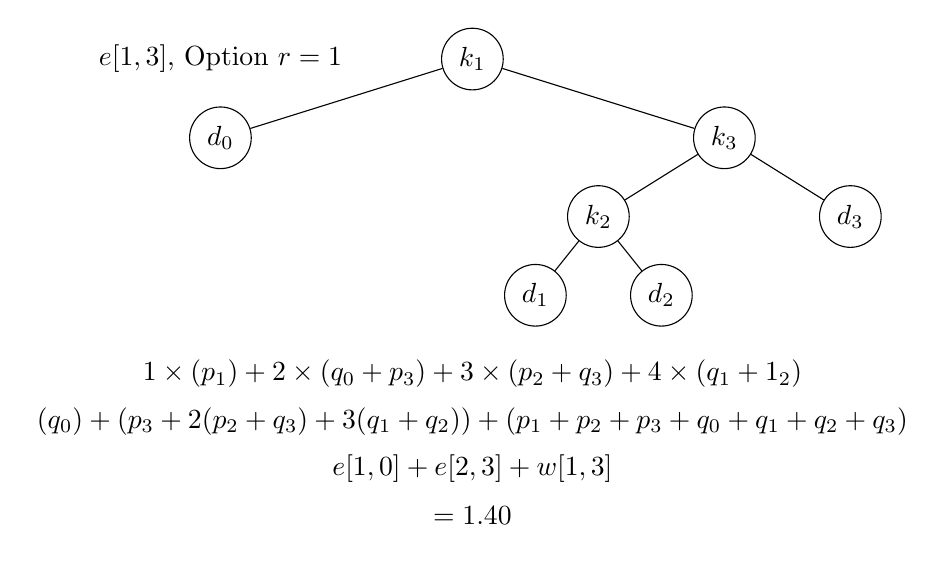
\begin{tikzpicture}[x=8mm, y=10mm]
	\node () at (-8,1) {$e[1,3]$, Option $r=1$};
	\node [circle, draw] (k1) at (-4,1) {$k_1$};
	\node [circle, draw] (k2) at (-2,-1) {$k_2$};
	\node [circle, draw] (k3) at (0,0) {$k_3$};
	\node [circle, draw] (d0) at (-8,0) {$d_0$};
	\node [circle, draw] (d1) at (-3,-2) {$d_1$};
	\node [circle, draw] (d2) at (-1,-2) {$d_2$};
	\node [circle, draw] (d3) at (2,-1) {$d_3$};
	\foreach \from/\to in {k3/k2, k3/d3, k2/d1, k2/d2, k1/d0, k1/k3}
		\draw (\from) -- (\to);
	\node () at (-4,-3) {$1\times (p_1) + 2\times (q_0 + p_3) + 3 \times (p_2 + q_3) + 4 \times (q_1 + 1_2)$};
	\node () at (-4,-3.6) {$ (q_0) +  (p_3 + 2(p_2+q_3) + 3(q_1 + q_2)) + (p_1 + p_2 + p_3 + q_0 + q_1 + q_2 + q_3)$};
	\node () at (-4,-4.2) {$e[1,0] + e[2,3] + w[1,3]$};
	\node () at (-4, -4.8) {$= 1.40$};
\end{tikzpicture}

\	

	\item Rooted at $k_2$.  This option has two single-$k$ subgraphs.  
	
	\
	
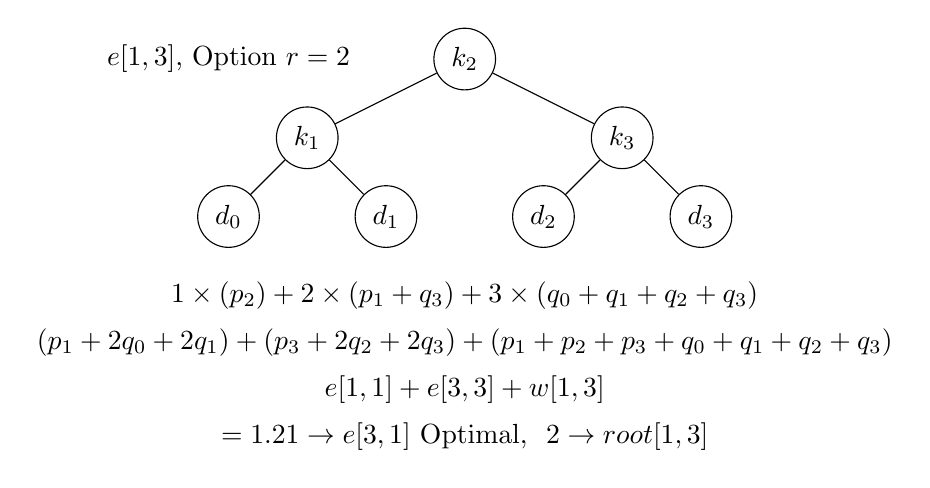
\begin{tikzpicture}[x=10mm, y=10mm]
	\node () at (-3,0) {$e[1,3]$, Option $r=2$};
	\node [circle, draw] (k1) at (-2,-1) {$k_1$};
	\node [circle, draw] (k2) at (0,0) {$k_2$};
	\node [circle, draw] (k3) at (2,-1) {$k_3$};
	\node [circle, draw] (d0) at (-3,-2) {$d_0$};
	\node [circle, draw] (d1) at (-1,-2) {$d_1$};
	\node [circle, draw] (d2) at (1,-2) {$d_2$};
	\node [circle, draw] (d3) at (3,-2) {$d_3$};
	\foreach \from/\to in {k2/k1, k2/k3, k1/d0, k1/d1, k3/d2, k3/d3}
		\draw (\from) -- (\to);
	\node () at (0,-3) {$1 \times (p_2) + 2 \times (p_1 + q_3) + 3 \times (q_0 + q_1 + q_2 + q_3)$};
	\node () at (0, -3.6) {$(p_1 + 2q_0 + 2q_1) + (p_3 + 2q_2 + 2q_3) + (p_1 + p_2 + p_3 + q_0 + q_1 + q_2 + q_3)$};
	\node () at (0, -4.2) {$e[1,1] + e[3,3] + w[1,3]$};
	\node () at (0, -4.8) {$=1.21 \to e[3,1]$ Optimal, \ $2 \to root[1,3]$};
\end{tikzpicture}

	

	\item Rooted at $k_3$.  
	\begin{itemize}
		\item Put subgraph 2.A above as the left subgraph of $k_3$.
		\item Put subgraph 2.B above as the left subgraph of $k_3$.
	\end{itemize}
	Either option adds the same overhead of pushing $k_1$, $k_2$, $d_0$, $d_1$, and $d_2$ down a level, putting $k_3$ at level 0, and putting $d_3$ at level 1, thus adding $p_1 + p_2 + q_0 + q_1 + q_2 + p_3 + 2\cdot q_3$ to the expected cost of the existing subgraph.  Since 2.B has a lower expected cost than 2.A, we do not need to consider 2.A.  
	

\

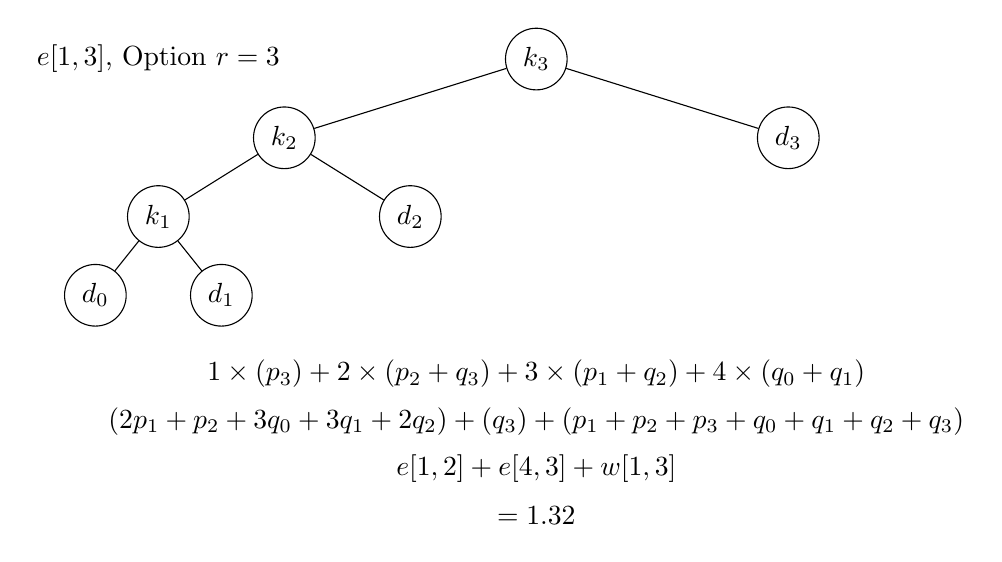
\begin{tikzpicture}[x=8mm, y=10mm]
	\node () at (-2,1) {$e[1,3]$, Option $r=3$};
	\node [circle, draw] (k1) at (-2,-1) {$k_1$};
	\node [circle, draw] (k2) at (0,0) {$k_2$};
	\node [circle, draw] (k3) at (4,1) {$k_3$};
	\node [circle, draw] (d0) at (-3,-2) {$d_0$};
	\node [circle, draw] (d1) at (-1,-2) {$d_1$};
	\node [circle, draw] (d2) at (2,-1) {$d_2$};
	\node [circle, draw] (d3) at (8,0) {$d_3$};
	\foreach \from/\to in {k2/k1, k2/d2, k1/d0, k1/d1, k3/k2, k3/d3}
		\draw (\from) -- (\to);
	\node () at (4,-3) {$1 \times (p_3) + 2 \times (p_2 + q_3) + 3 \times (p_1 + q_2) + 4 \times (q_0 + q_1)$};
	\node () at (4, -3.6) {$(2p_1 + p_2 + 3q_0 + 3q_1 + 2q_2) + (q_3) + (p_1 + p_2 + p_3 + q_0 + q_1 + q_2 + q_3)$};
	\node () at (4, -4.2) {$e[1,2] + e[4,3] + w[1,3]$};
	\node () at (4, -4.8) {$=1.32$};
\end{tikzpicture}

	
\end{itemize}

\

Continue adding layers.  

\


\begin{tabular}{ >{$}c<{$} | *7{c} }
e & 0 & 1 & 2 & 3 & 4 & 5 \cr\hline
1 & 0.04  & 0.28  & 0.70  & 1.21  & 1.89  & 2.70  \cr
2 &  & 0.05  & 0.33  & 0.81  & 1.38  & 2.16  \cr
3 &  &  & 0.06  & 0.38  & 0.92  & 1.57  \cr
4 &  &  &  & 0.07  & 0.43  & 1.04  \cr
5 &  &  &  &  & 0.08  & 0.49  \cr
6 &  &  &  &  &  & 0.09  \cr
\end{tabular}

\

\begin{tabular}{ >{$}c<{$} | *7{c} }
w & 0 & 1 & 2 & 3 & 4 & 5 \cr\hline
1 & 0.04  & 0.19  & 0.36  & 0.55  & 0.76  & 1.00  \cr
2 &  & 0.05  & 0.22  & 0.41  & 0.62  & 0.86  \cr
3 &  &  & 0.06  & 0.25  & 0.46  & 0.70  \cr
4 &  &  &  & 0.07  & 0.28  & 0.52  \cr
5 &  &  &  &  & 0.08  & 0.32  \cr
6 &  &  &  &  &  & 0.09  \cr
\end{tabular}

\

\begin{tabular}{ >{$}c<{$} | *7{c} }
root & 1 & 2 & 3 & 4 & 5 \cr\hline
1 & 1  & 2  & 2  & 3  & 4  \cr
2 &  & 2  & 3  & 3  & 4  \cr
3 &  &  & 3  & 4  & 4  \cr
4 &  &  &  & 4  & 5  \cr
5 &  &  &  &  & 5  \cr
\end{tabular}

\

Here's how to build the structure of the optimal binary tree from $root$.  

The element $root[1,5] = 4$ indicates that the subgraph of $k_1,\dots,k_5$, {\it i.e.} the entire graph, has $k_4$ as its root.  

If $k_4$ is the root, then $k_5$ is its right child, and its left child is the optimal subtree containing $k_1$, $k_2$, and $k_3$.  The element $root[1,3] = 2$ indicates that $k_2$ is the root of this subtree, implying that $k_1$ is its left child and $k_3$ is its right.  

Fill in the $d_i$'s.  

\

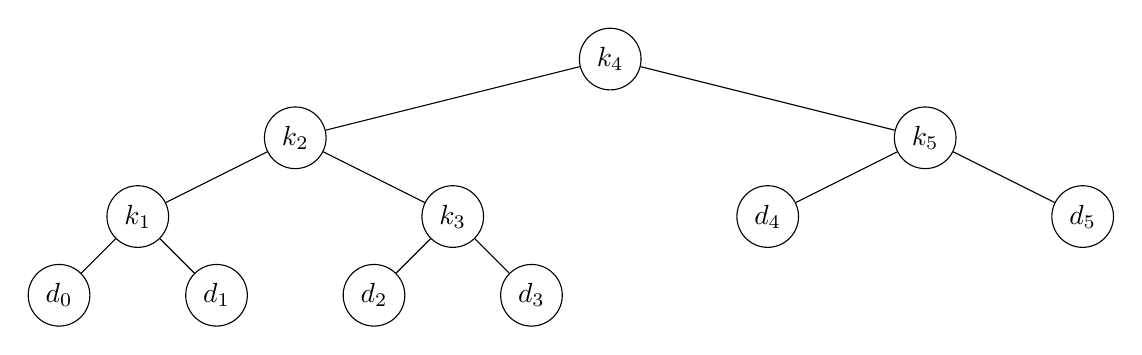
\begin{tikzpicture}[x=10mm, y=10mm]
	\node [circle, draw] (k1) at (-6,-2) {$k_1$};
	\node [circle, draw] (k2) at (-4,-1) {$k_2$};
	\node [circle, draw] (k3) at (-2,-2) {$k_3$};
	\node [circle, draw] (k4) at (0,0) {$k_4$};
	\node [circle, draw] (k5) at (4,-1) {$k_5$};
	\node [circle, draw] (d0) at (-7,-3) {$d_0$};
	\node [circle, draw] (d1) at (-5,-3) {$d_1$};
	\node [circle, draw] (d2) at (-3,-3) {$d_2$};
	\node [circle, draw] (d3) at (-1,-3) {$d_3$};
	\node [circle, draw] (d4) at (2,-2) {$d_4$};
	\node [circle, draw] (d5) at (6,-2) {$d_5$};
	\foreach \from/\to in {k4/k2, k4/k5, k2/k1, k2/k3, k5/d4, k5/d5, k1/d0, k1/d1, k3/d2, k3/d3}
		\draw (\from) -- (\to);
\end{tikzpicture}

\begin{align*}
	e[1,5] &= 1 \times (p_4) + 2 \times (p_2 + p_5) + 3 \times (p_1 + p_3 + q_4 + q_5) + 4 \times (q_0 + q_1 + q_2 + q_3) \cr
	&= 1(0.13)  + 2(0.11 + 0.15) + 3(0.10 + 0.12 + 0.08 + 0.09) + (0.04 + 0.05 + 0.06 + 0.07) \cr
	&= 1(0.13) + 2(0.26) + 3(0.39) + 4(0.22) \cr
	&= 0.13 + 0.52 + 1.17 + 0.88 \cr
	&= 2.70 \ \surd \cr
\end{align*}

\

Here's the code that takes in $n$, $p$, and $q$ and outputs the three tables in \LaTeX \ format.  

\lstinputlisting{OPTIMAL-BST.py}


%%%%%%%
\subsection{Old Exam Questions}
%%%%%
\subsubsection{S15 \#S9, Part (c)}

	% S15 \#S9
	Mark true/false against the following statements. 
	\begin{enumerate}[label=\alph*.]
		\item (Same as F15 \#S7a) A binary search tree of size $N$ will always find a key in at most $O(\log N)$ time.
		\item (Same as F15 \#S5c) A breadth first search algorithm can be considered as a special case of heuristic search algorithm.
		\item An optimal binary search tree is not necessarily a balanced tree.
		\item A dynamic programming approach uses top-down problem solving strategy to solve optimization problem.
	\end{enumerate}

\subsubsection{Solution to Part (c)}

True.  Minimizing the total expected cost may (probably will) require rotating things around to put the nodes of higher probability higher in the tree.  

%%%%%
\subsubsection{F15 \#S7, Part (b), Same as above}
	% F15 #S7
	Mark True or False against the following statements.
	\begin{enumerate}[label=\alph*.]
		\item  (Same as S15 \#9a) A binary search tree of size $N$ will always find a key in at most $O(\log N)$ time.
		\item An optimal binary search is not necessary a balanced tree.
		\item A binary heap always maintains a balanced tree as practical as it can be.
		\item To implement a priority queue binomial heap is preferred over binary heap.
		\item A graph formed by strongly connected components, a strongly connected components graph (SCC) is always a minimum spanning tree.  
	\end{enumerate}
	
%%%%%
\subsubsection{F16 \#S8, Third part, Same as above}
	% F16 #S8
	Mark true/false (T/F) against the following statements.  
	
	\begin{itemize}
		\item A binary search tree of size $N$ will always find a key at most $O(\lg N)$ time
		\item A breadth first search can be considered as a special case of heuristic search algorithm.
		\item An optimal binary search tree is not necessarily being a balanced tree.
		\item A dynamic programming approach uses top-down problem solving strategy to solve optimization problem.
	\end{itemize}



% Part (a) not yet solved.
\subsubsection{S15 \#L4}

	\begin{enumerate}[label=\alph*.]
		\item An object $r$ is accessed by its key $k_r$.  If all the objects have an equal chance of being accessed, what data structure will help you to have a better tight bound?  (State your assumptions and provide the bound you have obtained for the proposed structure.)
		\item An optimal binary search tree (\verb|OPTIMAL-BST|) for a given set of keys with known access probabilities ensures the minimum expected search cost for key accesses, with its pseudo code listed below.  Given the set of three keys with their access probabilities $k_1 = 0.25$, $k_2 = 0.15$, $k_3 = 0.3$, respectively, and four non-existing probabilities of $d_0 = 0.1$, $d_1 = 0.05$, $d_2 = 0.08$, $d_3 = 0.07$, construct optimal BST following dynamic programming with memorization for the given three keys and demonstrate the constructed optimal BST, which contains all three keys $(k_1, k_2, k_3)$ and four non-exististing dummies $(d_0, d_1, d_2, d_3)$.  (Show your work using the three tables for expected costs, $e[i,j]$, for access weights, $w[i,j]$, and for $root[i,j]$, with $i$ in $e[i,j]$ and $w[i,j]$ ranging from 1 to 4, $j$ in $e[i,j]$ and $w[i,j]$ ranging from 0 to 3, and both $i$ and $j$ in $root[i,j]$ ranging from 1 to 3.)
\

\verb|OPTIMAL-BST(p,q,n)|

\begin{lstlisting}[mathescape=true, numbers=left]
let $e[1..n+1, 0..n]$, $w[1..n+1, 0..n]$, and $root[1..n, 1..n]$ be new tables.
for $i=1$ to $n+1$
	$e[i, i-1] = q_{i-1}$
	$w[i, i-1] = q_{i-1}$
for $l=1$ to $n$
	for $i=1$ to $n-l+1$
		$j = i+l-1$
		$e[i,j] = \infty$
		$w[i,j] = w[i,j-1] + p_j + q_j$
		for $r=i$ to $j$
			$t = e[i,r-1] + e[r+1,j] + w[i,j]$
			if $t < e[i,j]$
				$e[i,j] = t$
				$root[i,j] = r$
return $e$ and $root$
\end{lstlisting}
\end{enumerate}

\

[Editor's Note] This question seems like it's supposed to be accessible (if tedious) to people who haven't worked with optimal binary search trees before, but it doesn't tell you what $p$ and $q$ are.  It should either say that $p_i = k_i$ and $q_i = d_i$, or it should use $p$ and $q$ instead of $k$ and $d$.  

\subsubsection{Solution to (a) TO DO}

Balanced binary search tree?


\subsubsection{Solution to (b)} \
	
	
\begin{tabular}{c|*6{c}}
e & 0 & 1 & 2 & 3 \cr\hline
1 & 0.10 &  0.55 &  1.14 &  2.15 &  \cr
2 & 0.00 &  0.05 &  0.41 &  1.13 &  \cr
3 & 0.00 &  0.00 &  0.08 &  0.60 &  \cr
4 & 0.00 &  0.00 &  0.00 &  0.07 &  \cr
\end{tabular}

\vskip 24pt

\begin{tabular}{c|*6{c}}
w & 0 & 1 & 2 & 3 \cr\hline
1 & 0.10 &  0.40 &  0.63 &  1.00 &  \cr
2 & 0.00 &  0.05 &  0.28 &  0.65 &  \cr
3 & 0.00 &  0.00 &  0.08 &  0.45 &  \cr
4 & 0.00 &  0.00 &  0.00 &  0.07 &  \cr
\end{tabular}

\vskip 24pt

\begin{tabular}{c|*6{c}}
root & 1 & 2 & 3 \cr\hline
1 & 1 &  1 &  2 &  \cr
2 & 0 &  2 &  3 &  \cr
3 & 0 &  0 &  3 &  \cr
\end{tabular}

\vskip 24pt

Here's how to read the \verb|root| array.  The element \verb|root[1][3] = 2| is the node at the root of the tree containing $k_1$, $k_2$, and $k_3$.  

\vskip 24pt

\begin{tikzpicture}[x=10mm, y=10mm]
	\node [circle, draw] (k1) at (-2,-1) {$k_1$};
	\node [circle, draw] (k2) at (0,0) {$k_2$};
	\node [circle, draw] (k3) at (2,-1) {$k_3$};
	\node [circle, draw] (d0) at (-3,-2) {$d_0$};
	\node [circle, draw] (d1) at (-1,-2) {$d_1$};
	\node [circle, draw] (d2) at (1,-2) {$d_2$};
	\node [circle, draw] (d3) at (3,-2) {$d_3$};
	\foreach \from/\to in {k2/k1, k2/k3, k1/d0, k1/d1, k3/d2, k3/d3}
		\draw [-triangle 60] (\from) -- (\to);
	\node [right] () at (4,0) {$1 \times (0.15)$};
	\node [right] () at (4,-1) {$2 \times (0.25 + 0.3)$};
	\node [right] () at (4,-2) {$3 \times (0.1 + 0.05 + 0.08 + 0.07)$};
	\node [right] () at (4,-3) {$0.15 + 1.10 + 0.9 = 2.15 = e[1][3] $};
\end{tikzpicture}



\subsection{F16 \#L4, Similar to above}

[Editor's Note:  In the copy that I have of the exam, the probabilities were blacked out.]

\

	Given a set of 4 keys, with the following probabilities, determine the cost and the structure of an optimal binary search tree, following the tabular, bottom-up method realized in the procedure of \verb|OPTIMAL-BST| below to construct and fill tables $e[1..5, 0..4]$, $w[1..5, 0..4]$, and $root[1..4, 1..4]$.  

\
		
	\hfil \begin{tabular}{c|ccccc}
		$i$ & 0 & 1 & 2 & 3 & 4 \cr\hline
		$p_i$ & & & & \cr
		$q_i$ & & & & \cr
	\end{tabular}

\
	
	\begin{lstlisting}[mathescape=true]
let $e[1..n + 1, 0..n ]$, $w[1..n+1, 0..n]$, and $root[1..n, 1..n]$ be new tables.
for $i=1$ to $n+1$
	$e[i, i-1] = q_{i-1}$
	$w[i, i-1] = q_{i-1}$
for $l=1$ to $n$
	for $i=1$ to $n-l+1$
		$j = i+l-1$
		$e[i,j] = \infty$
		$w[i,j] = w[,i,j-1] + p_j + q_j$
		for $r=i$ to $j$
			$t = e[i, r-1] + e[r+1,j] + w[i,j]$
			if $i<e[i,j]$
				$e[i,j] = t$
				$root[i,j] = r$
return $e$ and $root$
	\end{lstlisting}

\subsection{S17 \#L4, Similar to above}

	(Same as Fall 2016 \#L4 and S15 \#L4)


	 Given a set of 4 keys, with the following probabilities, determine the cost and the structure of an optimal BST (binary search tree), following the tabular, bottom-up method realized in the procedure of \verb|OPTIMAL-BST| below to construct and fill $e[1..5, 0..4], w[1..5,0..4]$ and $root[1..4,1..4]$.
	
\hfil	\begin{tabular}{>{$}r<{$}|ccccc}
		i & 0 & 1 & 2 & 3 & 4 \cr\hline
		p_i & & 0.10 & 0.08 & 0.22 & 0.21 \cr
		q_i & 0.06 & 0.12 & 0.07 & 0.05 & 0.09 \cr
	\end{tabular}
	
\

Construct and fill the three tables, and show the optimal BST obtained.  

\

\verb|OPTIMAL-BST(p,q,n)|

\begin{lstlisting}[mathescape=true, numbers=left]
let $e[1..n+1, 0..n]$, $w[1..n+1, 0..n]$, and $root[1..n, 1..n]$ be new tables.
for $i=1$ to $n+1$
	$e[i, i-1] = q_{i-1}$
	$w[i, i-1] = q_{i-1}$
for $l=1$ to $n$
	for $i=1$ to $n-l+1$
		$j = i+l-1$
		$e[i,j] = \infty$
		$w[i,j] = w[i,j-1] + p_j + q_j$
		for $r=i$ to $j$
			$t = e[i,r-1] + e[r+1,j] + w[i,j]$
			if $t < e[i,j]$
				$e[i,j] = t$
				$root[i,j] = r$
return $e$ and $root$
\end{lstlisting}

\subsubsection{Solution} \ 

\begin{tabular}{c|*6{c}}
e & 0 & 1 & 2 & 3 & 4 \cr\hline
1 & 0.06 &  0.46 &  0.95 &  1.62 &  2.44 &  \cr
2 & 0.00 &  0.12 &  0.46 &  1.05 &  1.79 &  \cr
3 & 0.00 &  0.00 &  0.07 &  0.46 &  1.19 &  \cr
4 & 0.00 &  0.00 &  0.00 &  0.05 &  0.49 &  \cr
5 & 0.00 &  0.00 &  0.00 &  0.00 &  0.09 &  \cr
\end{tabular}

\vskip 24pt

\begin{tabular}{c|*6{c}}
w & 0 & 1 & 2 & 3 & 4 \cr\hline
1 & 0.06 &  0.28 &  0.43 &  0.70 &  1.00 &  \cr
2 & 0.00 &  0.12 &  0.27 &  0.54 &  0.84 &  \cr
3 & 0.00 &  0.00 &  0.07 &  0.34 &  0.64 &  \cr
4 & 0.00 &  0.00 &  0.00 &  0.05 &  0.35 &  \cr
5 & 0.00 &  0.00 &  0.00 &  0.00 &  0.09 &  \cr
\end{tabular}

\vskip 24pt

\begin{tabular}{c|*5{c}}
root & 1 & 2 & 3 & 4 \cr\hline
1 & 1 &  1 &  2 &  3 &  \cr
2 & 0 &  2 &  3 &  3 &  \cr
3 & 0 &  0 &  3 &  4 &  \cr
4 & 0 &  0 &  0 &  4 &  \cr
\end{tabular}

\vskip 24pt

Here's how to use \verb|root| to find the structure of the table.  

The element $root[1,4] = 3$ gives the root node for the optimal binary search tree containing nodes $k_1, k_2, k_3$, and $k_4$.  So $k_3$ is at the root, which means $k_4$ is its right child.  The left subtree of $k_3$ contains $k_1$ and $k_2$.  The remaining question is how to structure that subtree.  The value of $root[1,2] = 1$ tells us that the subtree containing $k_1$ and $k_2$ has $k_1$ as its root.  Then fill in the $d$'s.  

\vskip 24pt

\begin{tikzpicture}[x=5mm, y=15mm]
	\node [circle, draw] (k1) at (-4,-1) {$k_1$}; 
	\node [circle, draw] (k2) at (-2,-2) {$k_2$}; 
	\node [circle, draw] (k3) at (0,0) {$k_3$}; 
	\node [circle, draw] (k4) at (4,-1) {$k_4$}; 
	\node [circle, draw] (d0) at (-6,-2) {$d_0$}; 
	\node [circle, draw] (d1) at (-3,-3) {$d_1$}; 
	\node [circle, draw] (d2) at (-1,-3) {$d_2$}; 
	\node [circle, draw] (d3) at (2,-2) {$d_3$}; 
	\node [circle, draw] (d4) at (6,-2) {$d_4$}; 
	\foreach \from/\to in {k3/k1, k3/k4, k1/d0, k1/k2, k4/d3, k4/d4, k2/d1, k2/d2}
		\draw [-triangle 60] (\from) -- (\to);

	\node [right] at (8,0) {$1 \times (p_3) = 1 \times (0.22) = 0.22$};
	\node [right] at (8,-1) {$2 \times (p_1 + p_4) = 2 \times (0.10 + 0.21) = 0.62$};
	\node [right] at (8,-2) {$3 \times (q_0 + p_2 + q_3 + q_4)$};
	\node [right] at (8.5,-2.4) {$= 3 \times (0.06 + 0.08 + 0.05 + 0.09) = 0.84$};
	\node [right] at (8,-3) {$4 \times (q_1 + q+2) = 4 \times (0.12 + 0.07) = 0.76$};
	\node [right] at (8,-4) {$0.22 + 0.62 + 0.84 + 0.76 = 2.44 = e[1,4]$};
\end{tikzpicture}

%%%%%
\subsubsection{F18 \#L1}

	% F18 #L1
	Describe how dynamic programming is used to construct an optimal binary search tree.  
	
	Use the following probability of $p$ and $q$, obtain the expected cost of searching an optimal binary search tree constructed by dynamic programming.  

	\
	
\hfil	\begin{tabular}{*9{|r}|}
		\hline
		$i$ & 0 & 1 & 2 & 3 & 4 & 5 & 6 & 7 \cr\hline
		$p_i$ & & 0.04 & 0.06 & 0.08 & 0.06 & 0.10 & 0.12 & 0.10 \cr\hline
		$q_i$ & 0.06 & 0.06 & 0.06 & 0.06 & 0.05 & 0.05 & 0.05 & 0.05 \cr\hline
	\end{tabular}
	
\

[Editor's Note] This is exercise 15.5-2, except that they changed two of the numbers.  It's different from other similar questions in the comps in that they didn't give us the code to follow.  

Why did they choose such a bloody long and tedious problem, where one calculation error can propagate through the entire problem?  They're just making more work for themselves grading it.  This is an $O(n^3)$ problem.  A problem with $n=4$ would have told them whether we knew how to do it.  

\subsubsection{Solution to the First Part} 

Four steps of developing a dynamic-programming algorithm.

\begin{enumerate}
	\item Characterize the structure of an optimal solution.
	\item Recursively define the value of an optimal solution.
	\item Compute the value of an optimal solution.
	\item Construct an optimal solution from computed information.  
\end{enumerate}

\subsubsection{Solution to the Second Part} \

\begin{tabular}{c|*9{c}}
e & 0 & 1 & 2 & 3 & 4 & 5 & 6 & 7 \cr\hline
1 & 0.06  & 0.28  & 0.62  & 1.02  & 1.43  & 1.95  & 2.56  & 3.14  \cr
2 &  & 0.06  & 0.30  & 0.68  & 1.01  & 1.53  & 2.08  & 2.63  \cr
3 &  &  & 0.06  & 0.32  & 0.65  & 1.08  & 1.60  & 2.15  \cr
4 &  &  &  & 0.06  & 0.28  & 0.65  & 1.09  & 1.59  \cr
5 &  &  &  &  & 0.05  & 0.30  & 0.72  & 1.12  \cr
6 &  &  &  &  &  & 0.05  & 0.32  & 0.72  \cr
7 &  &  &  &  &  &  & 0.05  & 0.30  \cr
8 &  &  &  &  &  &  &  & 0.05  \cr
\end{tabular}

\vskip 24pt

\begin{tabular}{c|*9{c}}
w & 0 & 1 & 2 & 3 & 4 & 5 & 6 & 7 \cr\hline
1 & 0.06  & 0.16  & 0.28  & 0.42  & 0.53  & 0.68  & 0.85  & 1.00  \cr
2 &  & 0.06  & 0.18  & 0.32  & 0.43  & 0.58  & 0.75  & 0.90  \cr
3 &  &  & 0.06  & 0.20  & 0.31  & 0.46  & 0.63  & 0.78  \cr
4 &  &  &  & 0.06  & 0.17  & 0.32  & 0.49  & 0.64  \cr
5 &  &  &  &  & 0.05  & 0.20  & 0.37  & 0.52  \cr
6 &  &  &  &  &  & 0.05  & 0.22  & 0.37  \cr
7 &  &  &  &  &  &  & 0.05  & 0.20  \cr
8 &  &  &  &  &  &  &  & 0.05  \cr
\end{tabular}

\vskip 24pt

\begin{tabular}{c|*9{c}}
root & 1 & 2 & 3 & 4 & 5 & 6 & 7 \cr\hline
1 & 1  & 2  & 2  & 3  & 3  & 3  & 4  \cr
2 &  & 2  & 3  & 3  & 3  & 5  & 5  \cr
3 &  &  & 3  & 3  & 4  & 5  & 5  \cr
4 &  &  &  & 4  & 5  & 5  & 6  \cr
5 &  &  &  &  & 5  & 6  & 6  \cr
6 &  &  &  &  &  & 6  & 6  \cr
7 &  &  &  &  &  &  & 7  \cr
\end{tabular}

\vskip 24pt

Here's how to use \verb|root| to build the tree.  

The value $root[1,7] = 4$ indicates that $k_4$ is the root of the subtree containing $k_1,\dots,k_7$, {\it i.e.} the entire tree.  

The left subtree contains $k_1, k_2$, and $k_3$, and the right subtree contains $k_5, k_6$ and $k_7$.

The root of the subtree containing $k_1$, $k_2$, and $k_3$ is $k_2$ because $root[1,3] = 2$.  Its left child is the subtree containing $k_1$, and its right child is the subtree containing $k_3$.  

The root of the subtree containing $k_5$, $k_6$, and $k_7$ is $k_6$ because $root[5,7] = 6$.  Its left child is the subtree containing $k_5$, and its right child is the subtree containing $k_7$.  

Add the dummy nodes.  

\

\begin{tikzpicture}[x=5mm, y=15mm]
	\node [circle, draw] (k1) at (-6,-2) {$k_1$};
	\node [circle, draw] (k2) at (-4,-1) {$k_2$};
	\node [circle, draw] (k3) at (-2,-2) {$k_3$};
	\node [circle, draw] (k4) at (0,0) {$k_4$};
	\node [circle, draw] (k5) at (2,-2) {$k_5$};
	\node [circle, draw] (k6) at (4,-1) {$k_6$};
	\node [circle, draw] (k7) at (6,-2) {$k_7$};
	\node [circle, draw] (d0) at (-7,-3) {$d_0$};
	\node [circle, draw] (d1) at (-5,-3) {$d_1$};
	\node [circle, draw] (d2) at (-3,-3) {$d_2$};
	\node [circle, draw] (d3) at (-1,-3) {$d_3$};
	\node [circle, draw] (d4) at (1,-3) {$d_4$};
	\node [circle, draw] (d5) at (3,-3) {$d_5$};
	\node [circle, draw] (d6) at (5,-3) {$d_6$};
	\node [circle, draw] (d7) at (7,-3) {$d_7$};
	\foreach \from/\to in {k4/k2, k4/k6, k2/k1, k2/k3, k6/k5, k6/k7, k1/d0, k1/d1, k3/d2, k3/d3, k5/d4, k5/d5, k7/d6, k7/d7}
		\draw [-triangle 60] (\from) -- (\to);
	\node [right] () at (8,0) {$1 \times (p_4) = 1 \times 0.06 = 0.06$};
	\node [right] () at (8,-1) {$2 \times (p_2 + p_6) = 2 \times (0.06 + 0.12) = 0.36$};
	\node [right] () at (8,-1.8) {$3 \times (p_1 + p_3 + p_5 + p_7)$};
	\node [right] () at (8.5,-2.2) {$= 3 \times (0.04 + 0.08 + 0.10 + 0.10) = 0.96$};
	\node [right] () at (-7,-3.8) {$4 \times (q_0 + q_1 + q_2 + q_3 + q_4 + q_5 + q_6 + q_7)$};
	\node [right] () at (-6.5,-4.2) {$= 4 \times (0.06 + 0.06 + 0.06 + 0.06 + 0.05 + 0.05 + 0.05 + 0.05) = 17.6$};
	\node [right] () at (-7,-5) {$0.06 + 0.36 + 0.96 + 1.76 = 3.14 = e[1,7]  $};
%	\node () at () {$$};
%	\node () at () {$$};
\end{tikzpicture}

%%%%%%%%%%%%%%%%%%
\section{Height Balanced Binary Search Tree (AVL Tree), \S 13, Problem 13-3}

\index{Binary Search Tree!Height Balanced!Definition, Problem 13-3}

An AVL Tree is a binary search tree that is {\bf height balanced}; that is, for each node, $x$, the heights of the left and right subtrees differ by at most 1.  

% Not finished.
\subsection{Old Exam Questions}
%%%%%
\subsubsection{S17 \#S1}
	% S17 #S1
	 \begin{enumerate}[label=\alph*.]
		\item Define height balanced binary tree.
		\item Write a pseudo code to determine whether a tree is height balanced?
		\item Obtain the tight bound of your algorithm.
	\end{enumerate}



\subsubsection{S18 \#S5, Same as above}
	% S18 #S5
	\begin{enumerate}[label=\alph*.]
		\item Define height balanced binary tree
		\item Write a pseudo code to determine whether a tree is height balanced?
		\item Obtain a tight bound of your algorithm.
	\end{enumerate}


